\chapter{Űrlap-vezérlőelemek használata}
\thispagestyle{empty}

A Calcban az adatok bevitelét látványosan megvalósíthatjuk
űrlapelemek segítségével. Az űrlapelemek
használatához be kell kapcsolni az
\textbf{Űrlap-vezérlőelemek} eszköztárat. Az
eszköztár első sorában találjuk a \textbf{Tervező mód
be/ki} kapcsolót, ami kikapcsolt állapotban a vezérlők
használatát, bekapcsolva pedig létrehozásukat és
módosításukat teszi lehetővé (\ref{ŰrlapVezérlőelemekA} ábra). 

\begin{figure}[h!]
\centering
\subfloat[Tervező mód be/ki]{\label{ŰrlapVezérlőelemekA}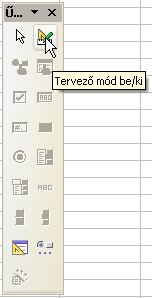
\includegraphics[width=.25\textwidth]{oocalcv2-img145.png}}
\qquad
\subfloat[Méret módosítása]{\label{ŰrlapVezérlőelemekB}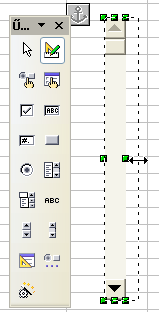
\includegraphics[width=.25\textwidth]{oocalcv2-img146.png}}
\caption{Űrlap-vezérlőelemek}\label{ŰrlapVezérlőelemek}
\end{figure}

A tervező módra váltva létrehozhatunk vezérlőket,
kiválasztva a megfelelő kapcsolót és az  átalakult
egérmutatóval megrajzolva a kívánt helyen, mint egy grafikai
objektumot. A létrehozott  vezérlőelem pozícióját és
méretét módosíthatjuk egér segítségével (\ref{ŰrlapVezérlőelemekB} ábra).
A Delete billentyűvel törölhetjük a kijelölt
vezérlőt.

\Aref{GyakranHasználtVezérlők} táblázat néhány gyakran használt
vezérlőt mutat be.

\begin{table}[!h]
\begin{center}
\caption{Gyakran használt vezérlők}\label{GyakranHasználtVezérlők}
\begin{tabular}{|m{1cm}|m{2.7cm}|b{8cm}|}
\hline
\multicolumn{1}{|c|}{\textbf{Ikon}}&
\multicolumn{1}{c|}{\textbf{Megnevezés}}&
\multicolumn{1}{c|}{\textbf{Leírás}} \\
\hline
\centering 
\includegraphics[width=0.741cm]{oocalcv2-img147.png} &
Jelölőnégyzet & Be- vagy kikapcsol egy műveletet az űrlapon.\\ \hline
\centering 
\includegraphics[width=0.741cm]{oocalcv2-img148.png} &
Rádiógomb & Több lehetőség közül választhatunk egyet.\\ \hline
\centering 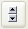
\includegraphics[width=0.741cm]{oocalcv2-img149.png} &
Léptetőgomb & Cellához rendelt értéket növelhetünk vagy csökkenthetünk
vele.\\ \hline
\centering 
\includegraphics[width=0.741cm]{oocalcv2-img150.png} &
Görgetősáv & Értéktartományt görget a görgetőnyilakra kattintva, vagy a
csúszkát elmozdítva.\\ \hline
\end{tabular}
\end{center}
\end{table}

Egy vezérlőelem létrehozása után be kell állítani
működési paramétereit. Ezeket a kijelölt vezérlőn a
\textbf{Vezérlés }paranccsal módosíthatjuk, amit a
gyorsmenüből vagy a Formátum eszköztárból érhetünk
el. \Aref{Görgetősáv} ábrán a görgetősáv vezérlőelem
tulajdonságok ablakának részletét látjuk. A minimális és
a maximális görgetési érték meghatározza, hogy a
vezérlő milyen értékeket ad annak a cellának aminek
címét --  az \textbf{Adat} fület választva --  beírunk.

\begin{figure}[!h]
\begin{center}
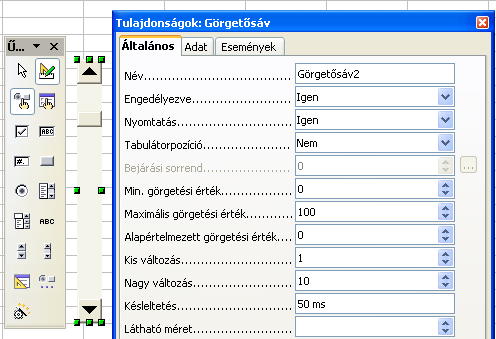
\includegraphics[width=12.253cm]{oocalcv2-img151.png}
\caption{Űrlap-vezérlőelemek --  Tulajdonságok: Görgetősáv}\label{Görgetősáv}
\end{center}
\end{figure}

A Jelölőnégyzet vezérlőelem segítségével logikai
IGAZ vagy HAMIS értéket állíthatunk be egy cellába.


\section{33. feladat}

{\itshape
Ábrázoljuk az $y=a\cdot x^{2}+b\cdot x+c$ függvény grafikonját
Pont(XY) diagramon. Az \textbf{a} értéke 1 és -1 közül
választható legyen rádiógombok segítségével. A \textbf{b}
és a \textbf{c} értéke gördítősávval módosítható
legyen -20 és 20 valamint -10 és 10 között. Számítsuk ki a
parabola csúcspontjának a koordinátáit is, de az értékek
megjelenítése jelölőnégyzettel kikapcsolható legyen.}

A függvény grafikonjának megépítéséhez először
hozzuk létre az x értékeket a C oszlopba -10-től 10-ig, 0,2
lépéssel. Az a, b és c értékek az F1, F2 és F3 cellába
kerülnek majd, írjunk ebbe a három cellába 1-et. A D oszlopba
számítsuk ki az y értékeket. A munkalap bal felső
részén hozzunk létre két rádiógombot. Az első
címkéje ,,a=1'' legyen a másodiké ,,a=-1''. A
háttérszín legyen 10\%-os szürke (\ref{33-feladat} ábra).

\begin{figure}[!h]
\begin{center}
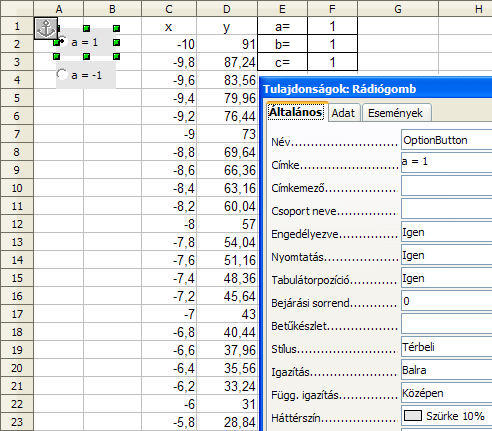
\includegraphics[width=12.016cm]{oocalcv2-img152.png}
\caption{33. feladat}\label{33-feladat}
\end{center}
\end{figure}

Az \textbf{Adat} fület választva a \textbf{Csatolt cella} sorba
írjunk F1-et, a \textbf{Referenciaérték (be)} legyen 1 (\ref{33-feladatRádiógomb}
ábra). A második rádiógomb csatolt cellája is az F1 legyen a
referenciaérték viszont -1.

\begin{figure}[!h]
\begin{center}
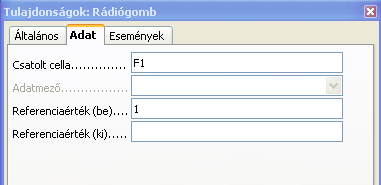
\includegraphics[width=10.081cm]{oocalcv2-img153.png}
\caption{33. feladat --  Tulajdonságok: Rádiógomb}\label{33-feladatRádiógomb}
\end{center}
\end{figure}

A tervező módot kikapcsolva próbáljuk ki a rádiógombok
működését. Az F1 cella tartalma a rádiógombokkal 1 és
-1 között választható. Amennyiben a függvény értéke nem
módosul a kapcsoló hatására, az annak a következménye, hogy
a rádiógomb szöveges értéket hoz létre az F1
cellában. Módosítani kell a függvény kiszámításának
képletét, az ÉRTÉK függvénnyel át kell alakítani a
szöveges értéket számmá. A módosított képletet \aref{33-feladatMódosított}.
ábrán látjuk.

\begin{figure}[!h]
\begin{center}
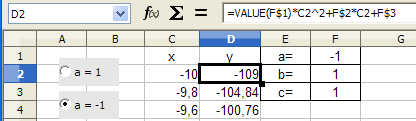
\includegraphics[width=11.005cm]{oocalcv2-img154.png}
\caption{33. feladat -- Módosított képlet}\label{33-feladatMódosított}
\end{center}
\end{figure}

Hozzuk létre a diagramot. Az Y és az X tengelyskálát
módosítsuk: minimum -20, maximum 20 és -10, 10. A
Főbeosztás mindkét esetben 1 legyen és kapcsoljuk is be
mindkettőt. Az X tengely feliratait forgassuk el 90 fokkal. A vonal
szélessége legyen 0,1 cm. 

A diagramtól balra hozzunk létre görgetősávot, ami a
\textit{c} értéket (az F3 cellát) módosítja -20-tól 20-ig
(\ref{33-feladatGörgetősáv} ábra).

\begin{figure}[!h]
\begin{center}
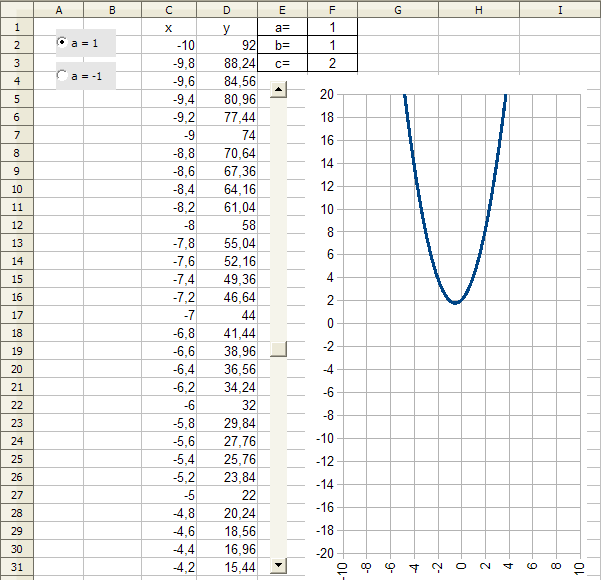
\includegraphics[width=14.9cm]{oocalcv2-img155.png}
\caption{33. feladat -- függőleges görgetősáv} \label{33-feladatGörgetősáv}
\end{center}
\end{figure}

A diagram alatt hozzunk létre egy vízszintes görgetősávot
ami a \textit{b }értéket (F2 cellát) módosítja -10 és 10
között.

A parabola csúcspontjának koordinátáit az 
$x_{0}=\frac{-{b}}{2\cdot a}$ és  $y_{0}=\frac{-b^{2}+4\cdot a\cdot
c}{4\cdot a}$ kifejezésekkel számíthatjuk ki. A koordináták
megjelenésének szabályzására hozzunk létre a
rádiógombok alatt jelölőnégyzetet. A címke legyen
,,A csúcspont koordinátái'',
engedélyezzük a szótörést, a csatolt cella az A50 legyen. A
HA függvény segítségével megoldhatjuk, hogy számérték
csak akkor jelenjen meg, ha a jelölőnégyzetet bekapcsoljuk.

A csúcspont y koordinátáját a következő képlettel
számíthatjuk ki:\\
{\sffamily\bfseries{=HA(A50;(-(F2\^{}2)+4*ÉRTÉK(F1)*F3)/(4*ÉRTÉK(F1));"")}}.

\Aref{33-feladatMegoldás} ábrán az elkészült feladatot látjuk. A
gördítősáv elmozdításával és a rádiógombokkal
egyszerűbb függvénytranszformációkat szemléltethetünk.

\begin{figure}[!h]
\begin{center}
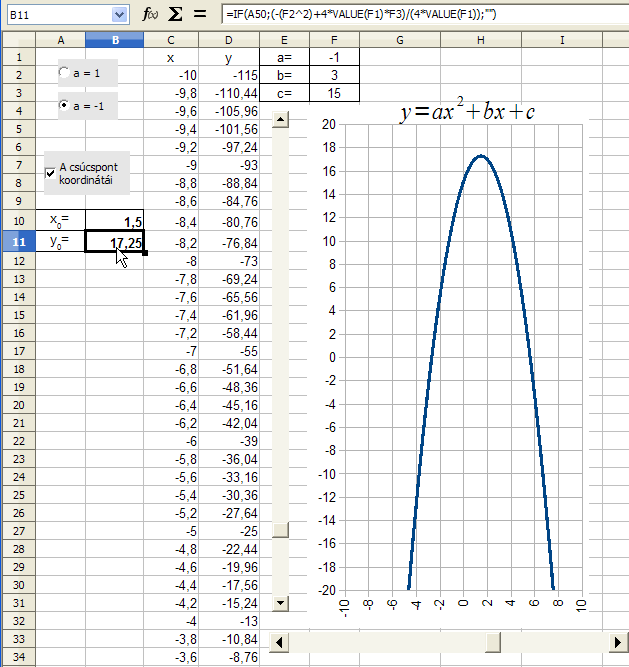
\includegraphics[width=15.999cm]{oocalcv2-img156.png}
\caption{33. feladat --  megoldás}\label{33-feladatMegoldás}
\end{center}
\end{figure}

